\section{Mexico City Prospective Study (MCPS)}

% ----------------------------------
% RECRUITMENT AND BASELINE DATA
% ----------------------------------
\subsection{Recruitment and baseline data}

% Overview -------------
\begin{frame}{Overview}
    \begin{columns}
        % Column with texth
        \begin{column}{0.45\textwidth}
            Over \highlight{150,000 participants} were recruited in two districts between \highlight{1998 and 2004}.
            \begin{itemize}
                \item Baseline questionnaire.
                \item Blood samples.
                \item Physical measurements.
                \item Linkage to mortality.
            \end{itemize}
            % Article title header
            \begin{figure}[htpb]
                \centering
                
\includegraphics[width=0.95\textwidth]{ziyatdinov2023/tapia-conyer2006_header.png}
            \end{figure}

        \end{column}
        % Columns with image
        \begin{column}{0.45\textwidth}
            \begin{figure}[htpb]
                \centering
                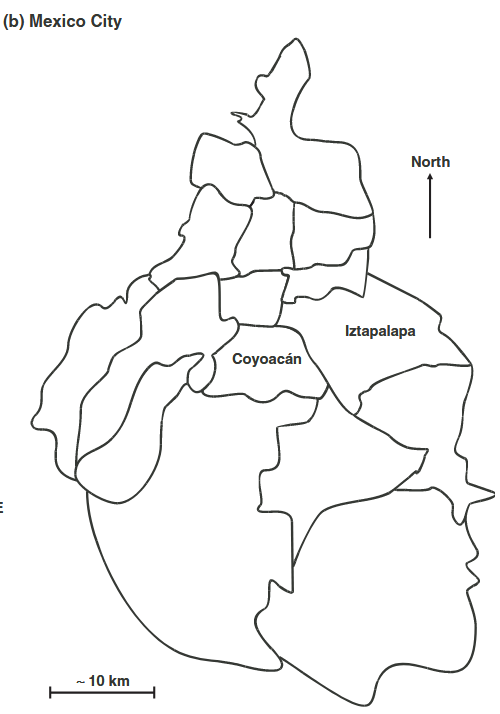
\includegraphics[width=0.45\textwidth]{ziyatdinov2023/map.png}
                \caption{Map showing the location of the MCPS districts \parencite{tapia-conyer-2006}.}
                \label{fig:mcps-main-map}
            \end{figure}
        \end{column}
    \end{columns}
\end{frame}

% Baseline data -------------
\begin{frame}{Baseline data}

    \vspace{-3mm}
    % Column A
    \begin{columns}[t]
        {\footnotesize
        \begin{column}{0.3\textwidth}

            % Socio-demographic - Textblock
            \begin{block}{Socio-demographic}<1->
                \begin{itemize}
                    \item Age and sex
                    \item Area of residence
                    \item Marital status
                    \item Educational achievement
                    \item Occupation
                    \item Income
                    \item Health service provider
                \end{itemize}
            \end{block}

            % Lifestyle - Textblock
            \begin{block}{Lifestyle characteristics}<2->
                \begin{itemize}
                    \item Diet (fruit/vegetables, fried food, types of oil)
                    \item Smoking and alcohol
                    \item Physical activity
                    \item Sleep duration
                \end{itemize}
            \end{block}

        \end{column}

        % Column B
        \begin{column}{0.3\textwidth}

            % Reproductive history - Textblock
            \begin{block}{Reproductive history (women)}<3->
                \begin{itemize}
                    \item Menopausal status
                    \item Hysteroctomy
                    \item Oopheroctomy
                    \item HRT
                    \item Contraceptive use
                    \item Pregnancy (age and number)
                \end{itemize}
            \end{block}

            % Physical measurements - Textblock
            \begin{block}{Physical measurements}<4->
                \begin{itemize}
                    \item Height
                    \item Weight
                    \item Waist and hip circumferece
                    \item Systolic and diastolic blood pressure
                \end{itemize}
            \end{block}

        \end{column}

        % Column C
        \begin{column}{0.3\textwidth}

            % Blood samples - Textblock
            \begin{block}{Blood samples}<5->
                \begin{itemize}
                    \item Plasma \& buffy coat
                    \item HbA1c and other essays
                    \item NMR metabolomics (e.g. fatty acids, cholines, lipoprotein subclasses, etc.)
                \end{itemize}
            \end{block}

            % Prior diseases and medications - Textblock
            \begin{block}{Prior diseases and medications}<6->
                Participants were asked if they had ever been diagnosed with any of the listed diseases (binary: \textit{Yes} or \textit{No}).
            \end{block}

        \end{column}
        }
    \end{columns}
\end{frame}

% ----------------------------------
% GENETIC OVERVIEW
% ----------------------------------
\subsection{Genetic overview}

% Genetic datasets ----------------
\begin{frame}{Genetic datasets}

    \begin{itemize}
        \item Genetic datasets were added later by \textcite{ziyatdinov2023}, making it one of the \highlight{largest} studies for \highlight{non-eurpean} populations.
        \item<2-> Comparison (WES and WGS) were made with other datasets: \textbf{UK Biobank}, \textbf{TOPMed}, \textbf{gnomAD}.
    \end{itemize}

    {\footnotesize
    \begin{columns}[t]

        \begin{column}{0.3\textwidth}
            \begin{block}{Genome-Wide Genotyping}<3->
                \begin{itemize}
                    \item Illumina --- GSAv2 chip array
                    \item 138,511 individuals
                \end{itemize}
            \end{block}
        \end{column}

        \begin{column}{0.3\textwidth}
            \begin{block}{Exome Sequencing (WES)}<4->
                \begin{itemize}
                    \item $n =$ 141,046 individuals
                \end{itemize}

                \textbf{Variants:}
                \begin{itemize}
                    \item \textit{Total:} 9.3 million.
                    \item \textit{Coding regions:} 4.0 million in 19,110 genes.
                    \item \textit{Unique MCPS:} 1.4 million.
                \end{itemize}

            \end{block}        
        \end{column}

        \begin{column}{0.3\textwidth}
            \begin{block}{Whole-Genome Sequencing (WGS)}<5->
                \begin{itemize}
                    \item $n =$ 9,950 individuals
                \end{itemize}

                \textbf{Variants:}
                \begin{itemize}
                    \item \textit{Total:} 131.9 million.
                    \item \textit{Coding regions:} 1.5 million.
                    \item \textit{Unique MCPS:} 31.5 million.
                \end{itemize}
            \end{block}
        \end{column}
    \end{columns}
    }

    \vfill

    \uncover<6->{
        \begin{itemize}
            \item Both \textbf{WES} and \textbf{WGS} share \alert{93.2\%} of the variants, with an increment of \alert{2.3\%} on \textbf{WGS} data.
        \end{itemize}
    }
\end{frame}

\begin{frame}{WES and WGS - Comparisons}

    \begin{itemize}
        \item Lower proportion of \highlight{singletons}, indicates \textit{extensive familial relatedness}.
        \item Increased number of \highlight{predicted loss of function (pLOF)} variants.
    \end{itemize}

    \medskip

    % Modified in Excel
    \begin{figure}[htpb]
        \centering
        % Supplementary Table 3
        \includegraphics<1>[width=0.95\textwidth]{ziyatdinov2023/table-comparison-3.png}
        % Supplementary Table 7
        \includegraphics<2>[width=0.95\textwidth]{ziyatdinov2023/table-comparison-7.png}
    \end{figure}
\end{frame}

% Family networks ----------------
\begin{frame}{Family networks}

\begin{columns}
    % Column 1
    \begin{column}{0.45\textwidth} 

       \begin{exampleblock}{Estimation}<1->
            Relatedness was estimated through \textit{identity-by-descent (IBD)} sharing.
       \end{exampleblock}

       \medskip
    
       \uncover<2->{
        About \alert{71\%} of individuals have \highlight{at least one relative} present in the MCPS dataset. 

       \begin{itemize}
           \item \textbf{Parent-Offspring (PO):} 31,597 relationships.
           \item \textbf{Sibling Pairs (FS):} 29,482 relationships.
           \item \textbf{Second Degree (2nd):} 47,080 relationships.
           \item \textbf{Third Degree (3rd):} 120,180 relationships.
       \end{itemize}
       }

    \end{column}
    % Column 2
    \begin{column}{0.45\textwidth}<3->
        \begin{figure}[htpb]
        \centering
        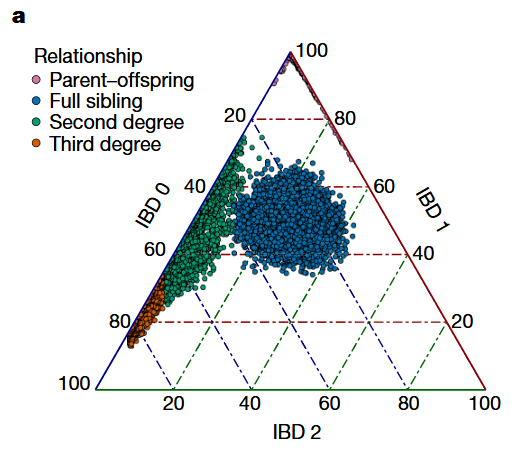
\includegraphics[width=0.95\textwidth]{ziyatdinov2023/familial-relatedness-a.png}
        \caption{Percentage of genome estimated to have zero, one or two IBD alleles \parencite{ziyatdinov2023}.}
        \label{fig:ibd-genome-percentage}
        \end{figure}
    \end{column}
\end{columns}
\end{frame}

\begin{frame}[t]{Family networks}
    \begin{figure}[htpb]
        \centering
        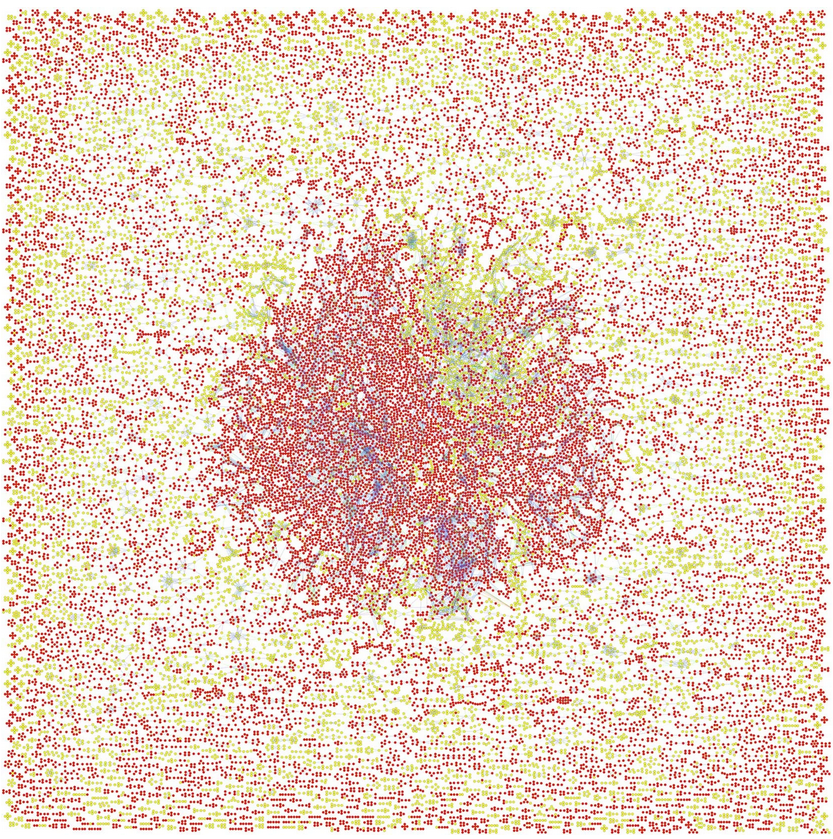
\includegraphics[height=2.25in]{ziyatdinov2023/2nd-degree-family-networks.png}
        \caption{Graph of second-degree family networks of size four or greater \parencite{ziyatdinov2023}.}
        \label{fig:2nd-degree-megaplot}
    \end{figure}
\end{frame}

\begin{frame}{Family networks}
    \begin{columns}
        % Column 1
        \begin{column}{0.5\textwidth}

            The levels of \textit{relatedness} were:
            \begin{itemize}
                \item much higher than those from the \textbf{UK Biobank (UKB)}.
                \item comparable with the \textbf{Geisinger Health Study (GHS)}--both \textbf{MCPS} and \textbf{GHS} recruited in \textit{close proximity}.
            \end{itemize}
        \end{column}

        % Image column -----
        \begin{column}{0.5\textwidth}
            \begin{figure}[htpb]
                \centering
                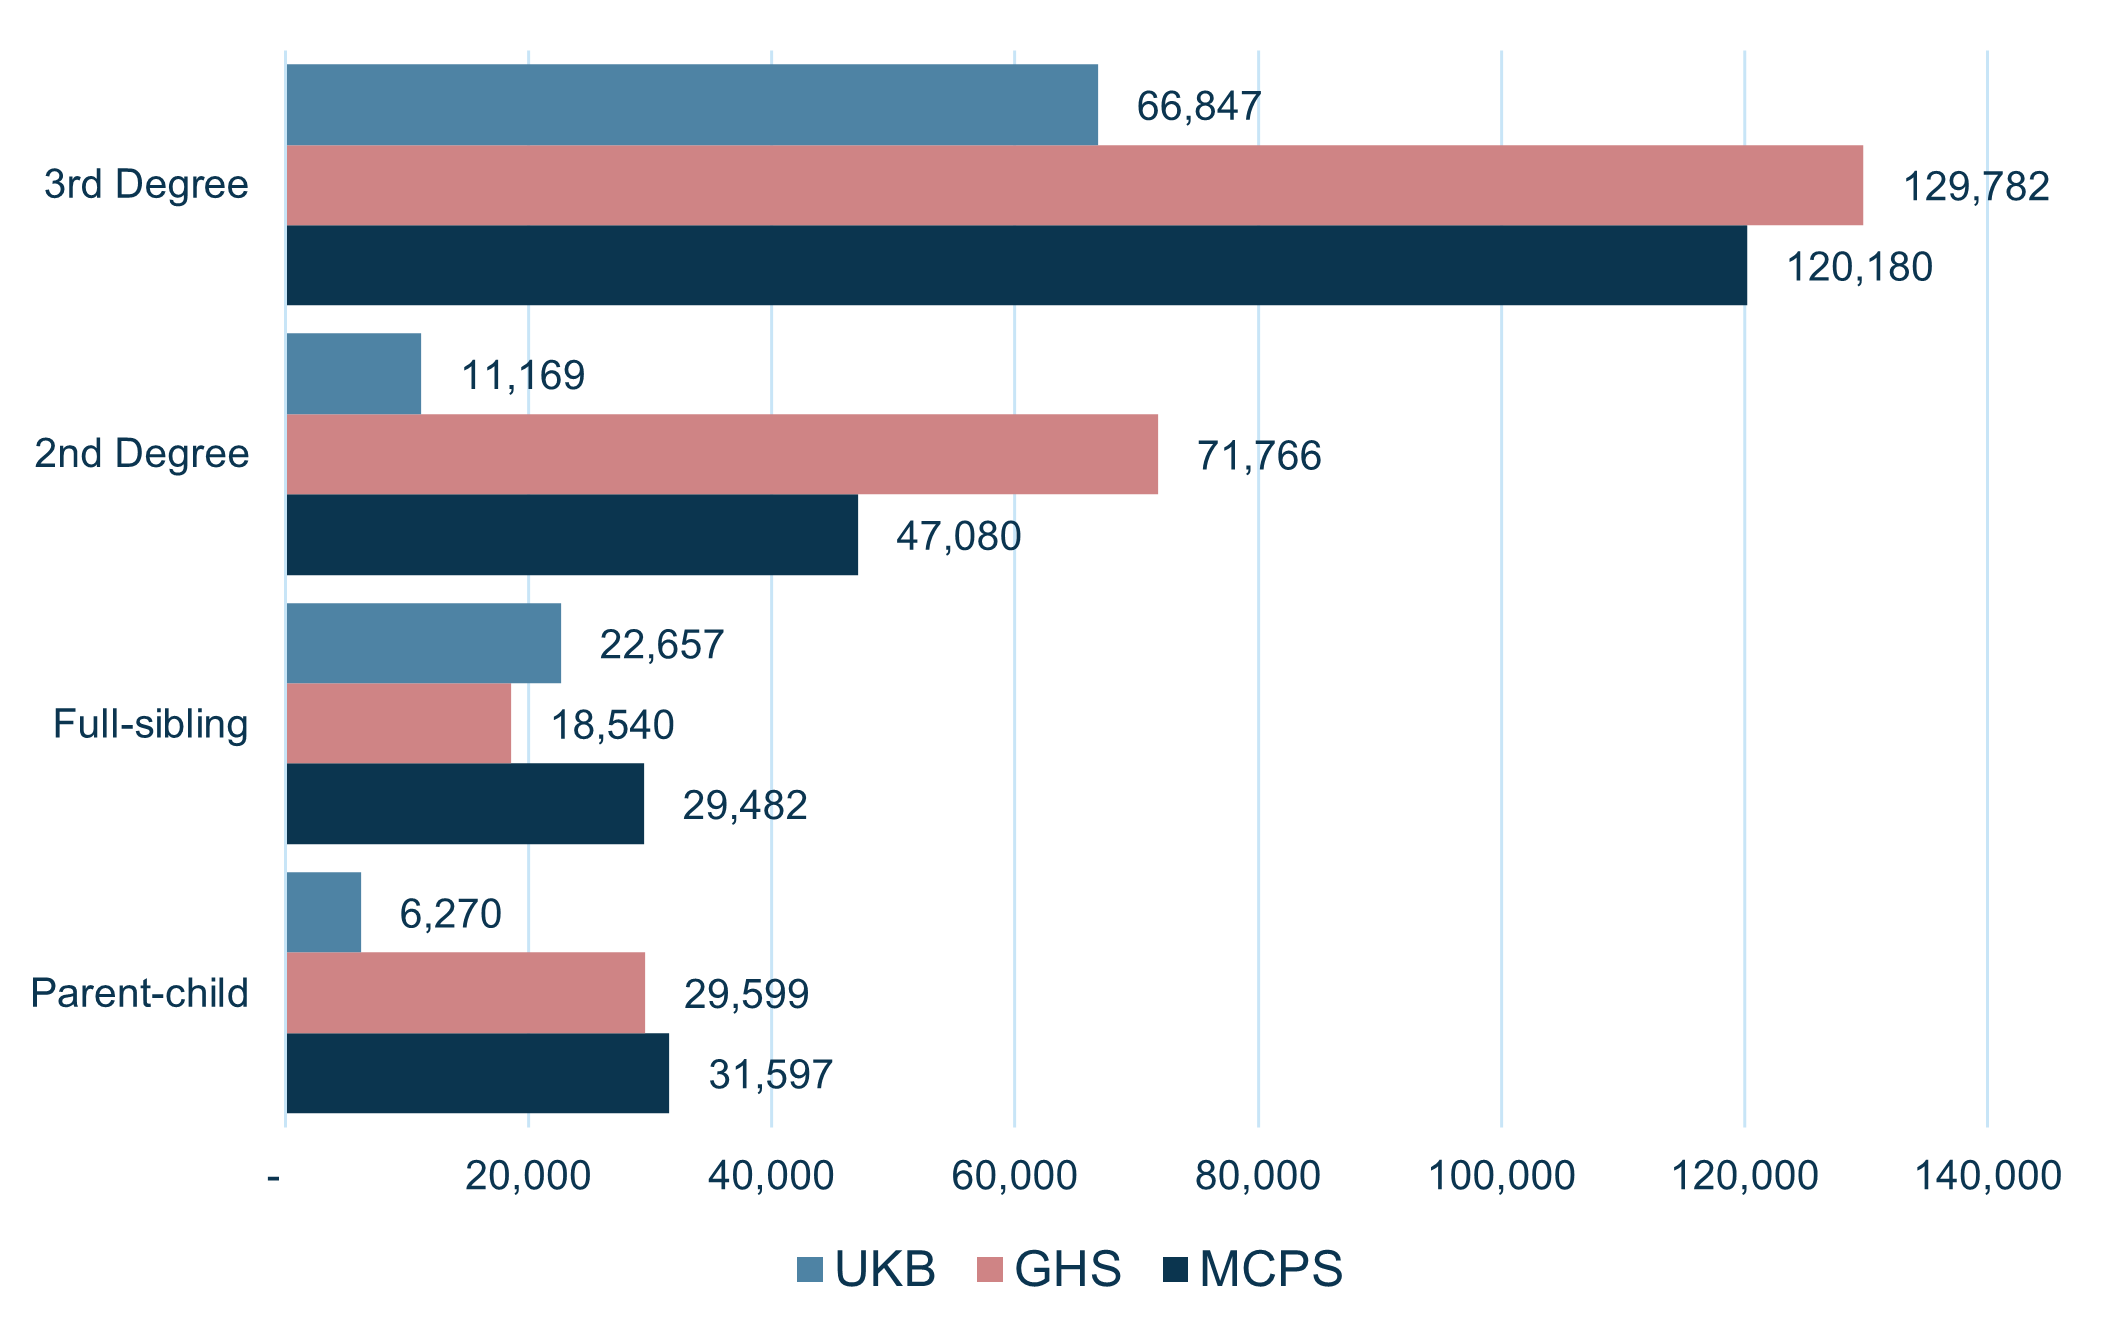
\includegraphics[width=0.95\textwidth]{ziyatdinov2023/dataset-comparison.png}
                \caption{Comparison of network sizes in MCPS, UKB and GHS. Data extracted from Supplementary Table 25 \parencite{ziyatdinov2023}.}
                \label{fig:ziyatdinov2023-nrelationships-comparison}
            \end{figure}
        \end{column}
    \end{columns}
\end{frame}

% Population structure -------------
\subsection{Population structure and ancestry}
\begin{frame}{Principal Components Analyses (PCA)}
\begin{columns}
    % Column 1
    \begin{column}{0.45\textwidth}

        Characterization of \alert{ancestry composition} adding \textit{unrelated} samples to PCA

        \begin{block}{1,000 Genomes Project}
            \begin{itemize}
                \item African (Yoruba): 108 samples
                \item European (Iberian): 107 samples
            \end{itemize}
        \end{block}
        \begin{block}{Metabolic Analysis of an Indigenous Samples (MAIS)}
            \begin{itemize}
                \item Indigenous Mexican: 591 samples (60 populations)
            \end{itemize}
            \parencite{garcia-ortiz2021}
        \end{block}
    \end{column}
    % Column 2
    \begin{column}{0.45\textwidth}
        \begin{figure}[htpb]
            \centering
            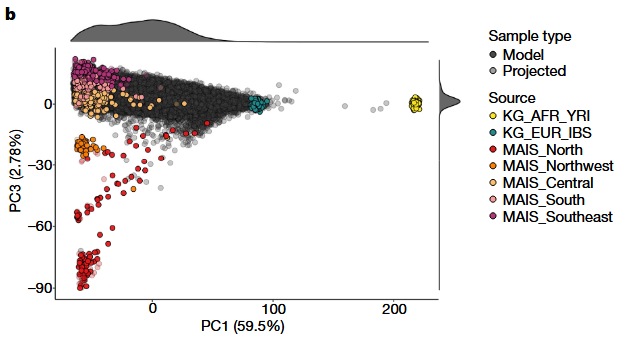
\includegraphics[width=0.95\textwidth]{ziyatdinov2023/pca-analysis.png}
            \caption{PCA for MCPS, African, European and Indigenous Mexican samples.}
            \label{fig:pca-1-ziyatdinov2023}
        \end{figure}
    \end{column}
\end{columns}

\end{frame}